\documentclass[aps,pra,reprint,superscriptaddress,amsmath,amssymb,longbibliography,floatfix]{revtex4-2}
\usepackage{amsthm}
\usepackage{bm,graphicx,booktabs}
\usepackage{xcolor}
\usepackage{hyperref}
\hypersetup{colorlinks=true,linkcolor=blue!45!black,citecolor=blue!45!black,urlcolor=blue!45!black,
  pdfauthor={Tingyu Zhang; Yan Cen}}
\newcommand{\ket}[1]{\lvert #1\rangle}
\newcommand{\bra}[1]{\langle #1\rvert}
\newcommand{\braket}[2]{\langle #1\mid #2\rangle}
\newcommand{\Tr}{\operatorname{Tr}}
\usepackage[T1]{fontenc}
\usepackage{microtype}
\newtheorem{theorem}{Theorem}
\newtheorem{lemma}{Lemma}
\newtheorem{proposition}{Proposition}
\begin{document}

\title{A unified construction of continuously tunable multiqubit elegant joint measurements}
\hypersetup{pdftitle={A unified construction of continuously tunable multiqubit elegant joint measurements}}
\author{Tingyu Zhang}
\email{23300190021@m.fudan.edu.cn}
\affiliation{Department of Physics, Fudan University, Shanghai, China}
\author{Yan Cen}
\email[Corresponding author: ]{cenyan@fudan.edu.cn}
\affiliation{Department of Physics, Fudan University, Shanghai, China}
\date{November 1, 2026}
\begin{abstract}
Continuous tuning of the common Bloch radius of an elegant joint measurement requires its local regular-tetrahedral geometry to remain compatible with a complete orthonormal measurement basis. This paper presents an explicit continuous family of elegant joint measurements for every integer $n\ge5$, using the same phase construction for odd and even $n$. The family passes through a specified reference measurement, preserves orthonormality and fixed local tetrahedral directions, and continuously covers the radius interval $[0,2r_E(n)]$, where $r_E(n)=\sqrt3/2^{n-1}$ is the reference radius. Within a fixed phase representation, a complete classification is obtained of the radius laws permitted by phase lines with two-valued real generators that pass through the reference measurement and preserve regular tetrahedral geometry with a common radius in its neighborhood. Consequently, the bound $2r_E(n)$ is attained and optimal within this model for every $n\ge5$, and $n=5$ is the smallest system size allowing radius enhancement in this model. For every even $n\ge8$, a two-dimensional measurement family is further constructed whose two coordinate sections recover the new enhanced family and the known cosine family column by column. The low-dimensional results further reveal the role of the phase path's shape: at $n=4$ in the same phase representation, even with arbitrary real phase generators, no phase line through the reference measurement that preserves the stated geometric conditions in its neighborhood can enhance the radius, whereas an explicit curved path reaches $(1+1/\sqrt2)r_E(4)$.

\end{abstract}
\maketitle
\section{Introduction}
\label{intro:section}

An entangled projective measurement is constrained both by the orthogonality of its global basis states and by the geometry of their local reductions. The elegant joint measurement (EJM) brings these two features together: the local Bloch vectors occupy the vertices of a regular tetrahedron, while the corresponding global states form an orthonormal basis. Introduced in the study of quantum networks~\cite{Gisin2017}, the EJM at $n=2$ belongs to a continuous family connecting it to a Bell-state measurement~\cite{Tavakoli2021}. Varying the tetrahedral radius changes the single-qubit reduced spectrum and hence the entanglement across each single-qubit-versus-rest cut. Extending this control to more qubits requires the local geometries of all measurement outcomes to remain compatible with global orthogonality.

Pauli-orbit constructions provide a useful setting for this problem~\cite{PauwelsPauli2026,PauwelsEJM2026}. In the associated phase normal form, every diagonal unitary generates a complete orthonormal basis; the remaining constraints concern the local Bloch vectors. Pauwels and Gisin gave an explicit reference EJM for every $n\ge2$, with common radius
\begin{equation}
 r_E(n)=\frac{\sqrt3}{2^{n-1}},
 \label{intro:reference-radius}
\end{equation}
and an even-qubit phase family with radius $r_E(n)\cos t$ on $|t|\le\pi/2$~\cite{PauwelsGisin2026}. Their construction already identifies interference involving a single computational-basis phase correction as the source of the local signal. Their odd-qubit analysis leaves an explicit tunable family through the specified reference point open for $n\ge5$, and identifies a locally isolated reference point at $n=3$ from a numerical Jacobian rank. Other symmetric multiqubit constructions permit broader local geometries~\cite{Ding2025,He2026}; here the target remains one fixed regular tetrahedron at each qubit, with a common radius across qubits and outcomes.

An earlier version of the present work supplied an explicit enhanced family for every odd $n\ge5$, with radius $r_E(n)(1-\sin t)$~\cite{Zhang2026Odd}. The present construction removes the odd--even distinction: a different Boolean kernel, depending on four binary features, gives the same radius law for every integer $n\ge5$. It recovers the reference measurement column by column at $t=0$ and continuously connects zero local polarization to twice the reference radius. This enhancement raises a natural question about its limit. We answer it for all two-valued real phase generators through the reference measurement by classifying the admissible radius laws. The doubled radius is optimal in this model, which includes generators beyond the four-feature construction.

The unified construction also makes it possible to compare the new enhancement with the known even-qubit cosine deformation within one phase representation. We examine whether both can be varied independently while preserving the local tetrahedra. For every even $n\ge8$, the answer is an explicit two-parameter family of complete measurements containing the two deformations as exact coordinate sections. At $n=6$, mixed interference obstructs this extension; in the corresponding four-color phase model, the local solutions consist of two crossing branches.

The lower-dimensional cases clarify why a straight phase path can cease to be sufficient. No two-valued phase line enhances the reference radius for $n=2,3,4$. At $n=3$, we strengthen the numerical evidence of Pauwels and Gisin to an exact local-rigidity certificate. At $n=4$, even allowing arbitrary real generators leaves every admissible straight line nonenhancing, but an explicit curved path increases the radius to $(1+1/\sqrt2)r_E(4)$. Thus the obstruction at $n=4$ can be overcome by changing the shape of the path within the same phase representation.

Section~II develops the phase framework that reduces these questions to local interference conditions. Sections~III and IV give the unified construction and its sharp Boolean-model bound. Section~V establishes its relation to the even-qubit family, and Sec.~VI explains the low-dimensional obstructions and the curved construction at $n=4$. The appendixes provide the full proofs.

\section{Phase framework and local geometry}
\label{core:framework}

To deform the local geometry while preserving an orthonormal measurement, we put the tunable parameters in a diagonal phase. For $n\ge2$, we use the computational basis $\ket{z_1\cdots z_n}$, with $z_j\in\mathbb F_2$, and the circuit convention of Ref.~\cite{PauwelsGisin2026}. Products act from right to left. Write
\begin{align}
 C_n&=S(n)H_n,\qquad M[D]=C_nDH^{\otimes n},\nonumber\\
 S(n)&=\mathrm{CNOT}_{2\to1}\cdots\mathrm{CNOT}_{n\to n-1},
 \label{core:phase-family}
\end{align}
where $H_n$ acts only on the last qubit and $D$ is diagonal with unit-modulus entries. By unitarity, the columns $\ket{\psi_k}=M[D]\ket{k}$ form a complete orthonormal measurement for every such $D$. Their local geometry is determined by the seed $\ket{\psi_0}$: writing $k=(e_1,\ldots,e_{n-1},\sigma)$ with $e\in\mathbb F_2^{n-1}$ and $\sigma\in\mathbb F_2$, the columns obey the exact Pauli orbit identity
\begin{equation}
 \ket{\psi_{e,\sigma}}=
 \left[\prod_{h=1}^{n-1}(Z_hZ_{h+1})^{e_h}\right]
 (X^{\otimes n})^\sigma\ket{\psi_0}.
 \label{core:orbit}
\end{equation}
This orbit propagates the seed's local Bloch vectors to all columns. To obtain regular tetrahedra with a common radius, it suffices to make the seed's signed local components equal. Our local coordinates are fixed throughout: only the final-qubit $Y$ component is sign-adjusted, $\widetilde Y_n=-Y_n$; every other $\widetilde P$ equals the corresponding physical Pauli operator. A common signed component $m\ge0$ therefore means seed Bloch vectors $m(1,1,1)$ for $j<n$ and $m(1,-1,1)$ for $j=n$.

We deform the reference phase
\begin{equation}
 \begin{aligned}
 f_0(z)&=\sum_{\ell=2}^n(-1)^\ell e_\ell(z)\\
 &=\begin{cases}0,&z=0,\\ |z|-1,&z\ne0,\end{cases}\pmod4.
 \end{aligned}
 \label{core:reference-phase}
\end{equation}
where $e_\ell$ is the elementary symmetric polynomial and $|z|$ is the Hamming weight. The reference measurement has $D_0(z)=i^{f_0(z)}$ and radius
\begin{equation}
 c_n=2^{1-n},\qquad r_E(n)=\sqrt3\,c_n.
 \label{core:reference-radius}
\end{equation}

To compute the seed's signed components, we separate a background state from a correction at the physical zero string. For any real function $\Theta$ on $\mathbb F_2^n$, set
\begin{align}
 \ket{\chi_\Theta}&=2^{-n/2}\sum_z i^{|z|}e^{i\Theta(z)}\ket z,\nonumber\\
 D_\Theta(z)&=\begin{cases}1,&z=0,\\
 i^{f_0(z)}e^{i\Theta(z)},&z\ne0.
 \end{cases}
 \label{core:background}
\end{align}
The seed is exactly
\begin{equation}
 \ket{\psi_0}=-iC_n\left[\ket{\chi_\Theta}
 +2^{-n/2}\big(i-e^{i\Theta(0)}\big)\ket{0^n}\right].
 \label{core:defect-state}
\end{equation}
The correction changes one physical input amplitude, irrespective of how $\Theta$ is represented.

\begin{lemma}[Local phase mechanism]
\label{core:mechanism}
For a signed local Pauli operator, write
\begin{equation}
 R=C_n^\dagger\widetilde P C_n=i^kX^aZ^b,\quad
 h=a\oplus b,\quad\Gamma=i^{k-|a|},
 \label{core:pauli-notation}
\end{equation}
and $B_R=\bra{\chi_\Theta}R\ket{\chi_\Theta}$. Then
\begin{equation}
 \langle\widetilde P\rangle
 =B_R+c_n\operatorname{Re}\!\left[
 \Gamma e^{-i\Theta(a)}\big(i-e^{i\Theta(0)}\big)\right].
 \label{core:signal}
\end{equation}
If all these signed expectations equal $m\ge0$, every measurement column has a true one-qubit reduced state
\begin{equation}
 \rho_{j,e,\sigma}
 =\frac12\left[I+\sqrt3m\,\mathbf v_{j,\kappa_j,\sigma}
 \cdot\boldsymbol\sigma\right],
 \label{core:bloch-orbit}
\end{equation}
where $e_0=e_n=0$, $\kappa_j=e_{j-1}\oplus e_j$, and
\begin{equation}
 \begin{aligned}
 \mathbf v_{j,q,s}&=\frac1{\sqrt3}
 \big((-1)^q,\epsilon_j(-1)^{q+s},(-1)^s\big),\\
 \epsilon_j&=\begin{cases}1,&j<n,\\-1,&j=n.\end{cases}
 \end{aligned}
 \label{core:vertices}
\end{equation}
For each $j$, these four unit vectors form a regular tetrahedron, and each label $(q,s)$ occurs $2^{n-2}$ times.
\end{lemma}

All pullbacks have $a\ne0$, so the correction in Eq.~\eqref{core:defect-state} has no diagonal contribution to a local expectation. Its two cross terms give Eq.~\eqref{core:signal}. Conjugation by the orbit operators in Eq.~\eqref{core:orbit} gives the tetrahedral signs in Eq.~\eqref{core:vertices}. Appendix~\ref{core:appendix} gives the pullbacks and the reduced-state derivation.

For the Boolean phase $\Theta=tq$, $q(0)=1$, the pullbacks fall into two classes: class I has $\Gamma=-i$ and $h\cdot a=1$, while class II has $\Gamma=-1$ and $h\cdot a=0$. With normalized Walsh coefficients
\begin{equation}
 \begin{aligned}
 W_q(h)&=2^{-n}\sum_z(-1)^{q(z)\oplus h\cdot z},\\
 D_aq(z)&=q(z)\oplus q(z\oplus a).
 \end{aligned}
 \label{core:walsh-def}
\end{equation}
the background is
\begin{equation}
 B_R(t)=\begin{cases}
 -\sin t\,W_q(h),&\text{class I},\\
 -\sin^2(t/2)\,W_{D_aq}(h),&\text{class II}.
 \end{cases}
 \label{core:boolean-background}
\end{equation}
These formulas express the background in terms of Walsh coefficients of the phase function and its derivatives.

\section{A unified family for all \texorpdfstring{$n\ge5$}{n >= 5}}
\label{core:unified}

Equation~\eqref{core:signal} suggests two design requirements: cancel every background term $B_R(t)$, and make the remaining cross terms equal. For Boolean phases, the first requirement gives the Walsh cancellations in Eq.~\eqref{core:boolean-background}, while the second fixes the values $q(a)$ at the local flips. For every integer $n\ge5$, four linear features reduce these requirements to conditions on one fixed four-bit kernel. Define the two internal parity blocks
\begin{equation}
 \begin{aligned}
 E_n&=\{2,4,\ldots\}\cap[2,n-2],\\
 O_n&=\{3,5,\ldots\}\cap[2,n-2],
 \end{aligned}
\end{equation}
and the four linear features
\begin{align}
 x&=z_1\oplus z_{n-1},& b&=\bigoplus_{j\in E_n}z_j,\nonumber\\
 c&=\bigoplus_{j\in O_n}z_j,& s&=z_1\oplus z_n.
 \label{core:features}
\end{align}
Write $\mathcal L_nz=(x,b,c,s)$. Both internal blocks are nonempty; the four features are independent. On $\mathbb F_2^4$, take
\begin{equation}
 F(x,b,c,s)=\begin{cases}
 1\oplus(1\oplus c)(x\oplus b),&s=0,\\
 b\oplus xc,&s=1.
 \end{cases}
 \label{core:kernel}
\end{equation}
Define
\begin{equation}
 q_n(z)=F(\mathcal L_nz),\qquad
 d_n(z)=q_n(z)-\delta_{z,0}.
 \label{core:support}
\end{equation}
Here the subtraction is in the integers. Since $F(0)=1$, $d_n$ is still Boolean. Only the physical zero string is removed, not the whole fiber $\mathcal L_nz=0$.

Figure~\ref{fig:unified}(a) shows how the same four-feature kernel determines the phase at every $n\ge5$; panel (b) displays the resulting radius in units of $r_E(n)$.
\begin{figure*}[tbp]
  \centering
  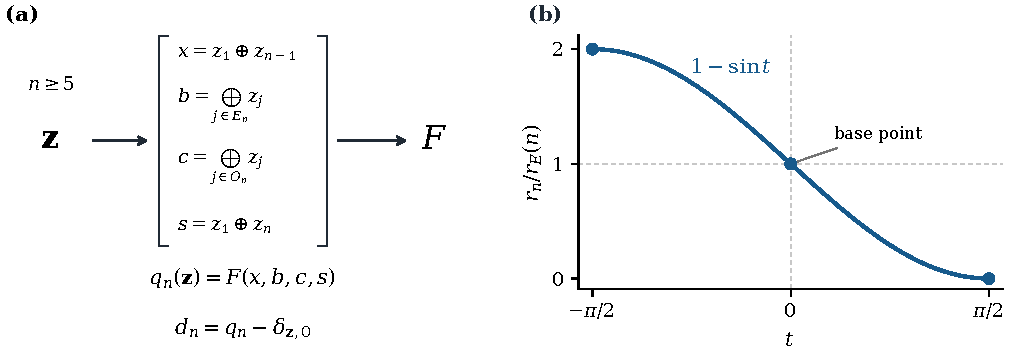
\includegraphics[width=\textwidth]{figures/fig1_unified.pdf}
  \caption{Unified phase deformation for every $n\geq5$.
  (a) Four linear Boolean features feed the same kernel $F$; the only removed support point is the physical string $\mathbf z=0$.
  The blocks $E_n$ and $O_n$ contain the even and odd indices in $[2,n-2]$, respectively.
  (b) The normalized common Bloch radius $r_n(t)/r_E(n)=1-\sin t$ on $[-\pi/2,\pi/2]$, where $r_E(n)=\sqrt3/2^{n-1}$ is the reference radius.
  From left to right, the marked points give the enhanced endpoint, the specified EJM at $t=0$, and the endpoint with maximally mixed one-qubit marginals.}
  \label{fig:unified}
\end{figure*}

\begin{theorem}[Unified enhanced family]
\label{core:unified-theorem}
For every integer $n\ge5$, let
\begin{equation}
 D_{n,t}(z)=i^{f_0(z)}e^{itd_n(z)},\qquad
 M_n(t)=C_nD_{n,t}H^{\otimes n}.
 \label{core:unified-measurement}
\end{equation}
For every real $t$, its columns are an orthonormal basis, and their one-qubit reduced states are Eq.~\eqref{core:bloch-orbit} with
\begin{equation}
 m_n(t)=c_n(1-\sin t),\qquad
 r_n(t)=r_E(n)(1-\sin t).
 \label{core:radius}
\end{equation}
The tetrahedral directions are independent of $t$. On
\begin{equation}
 J=[-\pi/2,\pi/2],\qquad r_n(J)=[0,2r_E(n)],
 \label{core:interval}
\end{equation}
the radius is continuous and strictly decreasing. At $t=0$, the reference measurement is recovered column by column; at $t=-\pi/2$ the radius is $2r_E(n)$, and at $t=\pi/2$ every one-qubit reduced state is $I/2$.
\end{theorem}

\begin{proof}
The proof separates the dimension-dependent feature map from six fixed four-bit cancellations. First, any sum of the form
\begin{equation}
 2^{-n}\sum_z(-1)^{h\cdot z}G(\mathcal L_nz)
 \label{core:pairing-sum}
\end{equation}
vanishes when $h$ is outside the row space of $\mathcal L_n$: a translation $z\mapsto z\oplus w$ with $\mathcal L_nw=0$ and $h\cdot w=1$ reverses each summand's sign. Inside that row space, write $h=\mathcal L_n^TH$. Equal fiber sizes reduce Eq.~\eqref{core:pairing-sum} to $2^{-4}\sum_v(-1)^{H\cdot v}G(v)$. The same argument applies to a derivative of $q_n$, since $D_aq_n=(D_AF)\circ\mathcal L_n$ with $A=\mathcal L_na$.

Second, the local characters in the pullback table leave only
\begin{align}
 W_F(9)&=W_F(11)=W_F(15)=0,\nonumber\\
 W_{D_6F}(6)&=W_{D_7F}(13)=W_{D_7F}(11)=0.
 \label{core:six-cancellations}
\end{align}
Integers encode $(x,b,c,s)$ with $x$ the most significant bit; the Walsh normalization is $2^{-4}$. The six sums vanish by pairing over feature bits. Appendix~\ref{core:alln-classification} gives the finite calculation and proves that these six identities cover every local component for all $n\ge5$, including the additional residual terms at $n=5,6,7$. Equation~\eqref{core:boolean-background} therefore gives $B_R(t)=0$ identically.

Third, every class-I flip satisfies $F(\mathcal L_na)=0$, and every class-II flip satisfies $F(\mathcal L_na)=1$. Equation~\eqref{core:signal} therefore reduces, respectively, to
\begin{align}
 c_n\operatorname{Re}[-i(i-e^{it})]&=c_n(1-\sin t),\nonumber\\
 c_n\operatorname{Re}[-e^{-it}(i-e^{it})]&=c_n(1-\sin t).
\end{align}
Lemma~\ref{core:mechanism} transfers this seed identity to all measurement columns. The endpoint, base-point, and image statements follow from the diagonal phase and the strict monotonicity of $\sin t$ on $J$.
\end{proof}

The enhancement has a direct one-qubit entanglement interpretation. All outcomes and all $1|(n-1)$ cuts share the spectrum
\begin{equation}
 \lambda_\pm=\frac{1\pm r_n(t)}2,
 \qquad \operatorname{Tr}\rho_j^2=\frac{1+r_n(t)^2}{2}.
 \label{core:spectrum}
\end{equation}
Their entropy is $h_2((1+r_n(t))/2)$, where $h_2(p)=-p\log_2p-(1-p)\log_2(1-p)$ with its continuous endpoint values. Increasing the Bloch radius decreases this bipartite entanglement. At $t=\pi/2$, the point correction in Eq.~\eqref{core:defect-state} vanishes; at $t=-\pi/2$, its interference produces twice the reference local signal. Four linear features suffice to express the phase for all $n$, while the feature extraction itself still depends on the physical register size.






\section{Sharp bounds for Boolean phase lines}
\label{bound:section}

The enhanced family also attains the largest radius possible for a broader
class of phase deformations generated by real functions taking at most
two values on the physical input strings; constant generators are included.
Subtracting the generator's value at $z=0$ removes a global phase.
A constant generator then becomes zero; otherwise, rescaling or reversing
$t$ makes the two values $0$ and $1$. We can therefore use a Boolean
generator, without a compression assumption or a condition on the
background state, and write
\begin{equation}
 \begin{gathered}
 M_d(t)=C_n\operatorname{diag}_{z}
 \bigl(i^{f_0(z)}e^{itd(z)}\bigr)H^{\otimes n},\\
 d:\mathbb F_2^n\longrightarrow\{0,1\},\qquad d(0)=0.
 \end{gathered}
 \label{bound:line}
\end{equation}
We call such a line admissible if, on an open interval containing $t=0$,
its local Pauli orbits form regular tetrahedra with a common radius.
This requirement refers to the complete measurement.  The unitary
factorization already guarantees orthonormality for every real $t$.

When the signed local components share a value $m_d(t)$, the common
Bloch radius is
\begin{equation}
 r_d(t)=\sqrt3\,|m_d(t)|.
 \label{bound:radius}
\end{equation}
Intervals with $m_d\ge0$ retain the original tetrahedral orientation.

\begin{theorem}[Four laws and the sharp Boolean-line bound]
\label{bound:theorem}
Let $n\ge3$ and let $d$ be admissible.  Set $c_n=2^{1-n}$.
All signed local components have one common value $m_d(t)$ for every
real $t$, and, for one fixed pair $(s,k)\in\{0,1\}^2$,
\begin{equation}
 m_d(t)=c_n\bigl[(1-s)+s\cos t-k\sin t\bigr].
 \label{bound:four-laws}
\end{equation}
Thus the four possible functional forms of $m_d/c_n$ are
$1$, $\cos t$, $1-\sin t$, and $\cos t-\sin t$.
Not every form occurs in every dimension.
For every $n\ge2$, with $r_E(n)=\sqrt3\,c_n$, the exact maximum over admissible lines is
\begin{equation}
 \max_{\substack{d\ \text{admissible}\\t\in\mathbb R}}r_d(t)
 =\begin{cases}
 r_E(n),&n=2,3,4,\\
 2r_E(n),&n\ge5.
 \end{cases}
 \label{bound:sharp-max}
\end{equation}
Both maxima are attained.
\end{theorem}

At the base point all these components equal $c_n>0$.
Regularity therefore makes them equal on a neighborhood of the base
point.  Each component is a linear combination of $1$, $\cos t$, and
$\sin t$, so equality on that neighborhood implies equality for all
real $t$.

The essential restriction comes from comparing coefficients for the two
classes of pulled-back Pauli operators.  Put $q=d+\delta_0$, so that
$q$ is Boolean and $q(0)=1$, and use the Walsh coefficients and Boolean
derivatives defined in Eq.~\eqref{core:walsh-def}.
For class I, the coefficient of $\cos t$ is $c_nq(a)$; for class II,
the coefficient of $\sin t$ is $-c_nq(a)$.  Since both classes occur
for $n\ge3$, equality of the components forces a common flip value
$s$ in class I and a common flip value $k$ in class II.  The remaining
coefficients agree precisely when
\begin{equation}
 \begin{aligned}
 q(a)&=s,& W_q(h)&=c_n(s+k-1)&&({\rm I}),\\
 q(a)&=k,& W_{D_aq}(h)&=2c_n(s+k-1)&&({\rm II}).
 \end{aligned}
 \label{bound:conditions}
\end{equation}
These conditions give Eq.~\eqref{bound:four-laws} and are also
sufficient.  For the enhanced law $1-\sin t$, they force both Walsh
coefficients to vanish, so Eq.~\eqref{core:boolean-background} makes the
background identically zero.

The maximum absolute values of the four normalized functions are,
respectively, $1$, $1$, $2$, and $\sqrt2$.  This proves the upper bound
$2r_E$ for every $n\ge3$.  The low-dimensional restrictions are stronger.
For $n=3$, two class-I character equations force $s=k=0$.
For $n=4$, four such equations sum to $4k=0$, leaving only the constant
and cosine laws.  The calculation for $n=2$, where class II is absent,
also permits only these two laws.  Appendix~\ref{bound:appendix}
gives the coefficient calculation and these analytic exclusions.
The base point attains the low-dimensional maximum, while the unified
family attains $2r_E$ at $t=-\pi/2$ for every $n\ge5$.

Consequently, $n=5$ is the smallest system size permitting an
increase of the radius along a phase line through the specified base
point with a two-valued real generator. General multivalued phase lines
and curved paths require a separate analysis; the case $n=4$ below
makes this distinction concrete.

\section{Embedding the even-qubit family}
\label{embed:section}

The unified construction and the earlier even-qubit family provide two phase directions through the same reference measurement. We now ask whether both directions can be varied independently while preserving the tetrahedral geometry. To compare them at the level of the complete measurement, first express the earlier family in the notation of Sec.~\ref{core:framework}. For even $n$, retain
$E_n=\{2,4,\ldots,n-2\}$ and define
\begin{equation}
 q_A(z)=\prod_{j\in E_n}(1-z_j),\qquad d_A(z)=q_A(z)-\delta_{z,0}.
 \label{embed:and-support}
\end{equation}
The diagonal $i^{f_0(z)}e^{i\alpha d_A(z)}$ is precisely the even-qubit family of Pauwels and Gisin~\cite{PauwelsGisin2026}, with $\alpha=\pi\tau/2$ in their parameter convention. Its background depends only on the even internal coordinates. Every character $h$ in Table~\ref{core:pullback-table} contains a coordinate outside $E_n$, so a flip of that coordinate cancels the background expectation. Moreover, $q_A(a)=1$ for class I and $q_A(a)=0$ for class II. Equation~\eqref{core:signal} then gives the common signed component $c_n\cos\alpha$, and hence $r=r_E(n)\cos\alpha$ for $|\alpha|\le\pi/2$. This argument includes $n=2$, where the product is empty and $q_A=1$, and $n=4$, where $q_A=1-z_2$.

For even $n\ge8$, this family and the unified enhanced family are coordinate sections of a two-parameter family. Write $d_B=d_n$ for the support in Eq.~\eqref{core:support} and set
\begin{align}
 D_{\alpha,\beta}(z)&=i^{f_0(z)}e^{i\alpha d_A(z)+i\beta d_B(z)},\notag\\
 M_n(\alpha,\beta)&=C_nD_{\alpha,\beta}H^{\otimes n}.
 \label{embed:measurement}
\end{align}
Figure~\ref{fig:embedding} shows the two-parameter family and its coordinate sections.
\begin{figure*}[tbp]
  \centering
  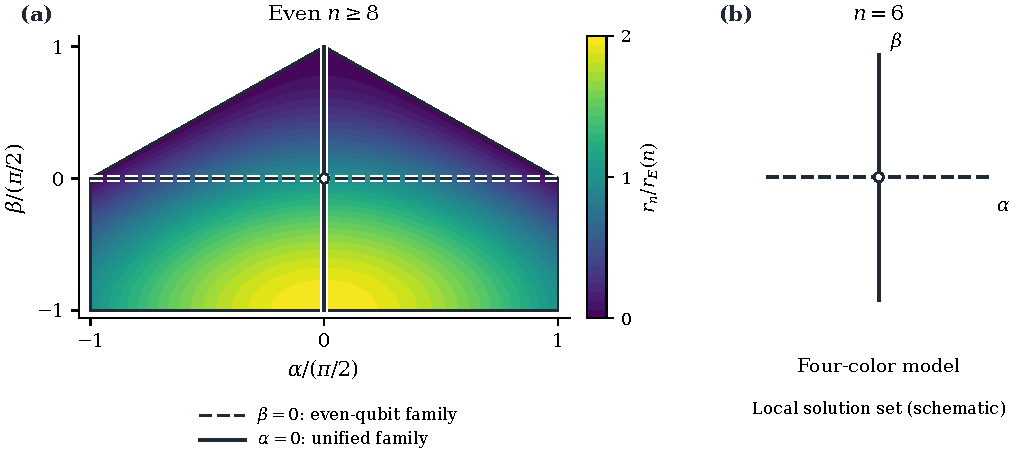
\includegraphics[width=\textwidth]{figures/fig2_embedding.pdf}
  \caption{Two exact sections of an even-qubit two-parameter family.
  (a) For even $n\geq8$, the domain $\Omega$ is given by $|\alpha|\leq\pi/2$ and $-\pi/2\leq\beta\leq\pi/2-|\alpha|$.
  Color represents $r_n/r_E(n)=\cos\alpha-\sin\beta$, with reference radius $r_E(n)=\sqrt3/2^{n-1}$; both axes are in units of $\pi/2$.
  The dashed section $\beta=0$ recovers the prior even-qubit cosine family, and the solid section $\alpha=0$ recovers the unified enhanced family, in each case column by column.
  The open circle marks the common base point.
  (b) Schematic local solution set at $n=6$ in the four-color model, with phases assigned to the four values of $(q_A,q_B)$ and an independent zero-string phase: the two branches cross at the base point.}
  \label{fig:embedding}
\end{figure*}

\begin{theorem}[Two-parameter embedding]
\label{embed:theorem}
For every even $n\ge8$, Eq.~\eqref{embed:measurement} defines an orthonormal measurement for all real $\alpha,\beta$. All its signed seed components equal
\begin{equation}
 m_n(\alpha,\beta)=c_n(\cos\alpha-\sin\beta).
 \label{embed:component}
\end{equation}
On the domain
\begin{equation}
 \Omega=\left\{(\alpha,\beta): |\alpha|\le\frac\pi2,\quad
 -\frac\pi2\le\beta\le\frac\pi2-|\alpha|\right\},
 \label{embed:domain}
\end{equation}
the measurement has the fixed local tetrahedra of Eq.~\eqref{core:bloch-orbit}, with
\begin{align}
 r_n(\alpha,\beta)&=r_E(n)(\cos\alpha-\sin\beta),\notag\\
 r_n(\Omega)&=[0,2r_E(n)].
 \label{embed:radius}
\end{align}
Its $\beta=0$ section recovers the earlier even-qubit family column by column, and its $\alpha=0$ section recovers Theorem~\ref{core:unified-theorem} column by column. The two parameter directions are independent as ordered measurement projectors.
\end{theorem}

The essential step is cancellation of the joint background. Put $u=e^{i\alpha}$ and $v=e^{i\beta}$. The seed before applying $-iC_n$ is
\begin{equation}
 2^{-n/2}\left[\sum_z i^{|z|}u^{q_A(z)}v^{q_B(z)}\ket z
 +(i-uv)\ket{0^n}\right],
 \label{embed:seed}
\end{equation}
where $q_B=q_n$. At every class-I flip, $(q_A(a),q_B(a))=(1,0)$; at every class-II flip, the pair is $(0,1)$. Their defect contributions therefore agree, because
\begin{align}
 \operatorname{Re}[-iu^{-1}(i-uv)]
 &=\cos\alpha-\sin\beta,\notag\\
 \operatorname{Re}[-v^{-1}(i-uv)]
 &=\cos\alpha-\sin\beta.
 \label{embed:defect}
\end{align}
Class I leaves $q_A$ unchanged, reducing its background to the already vanishing $q_B$ background. In class II, the AND difference separates the background sum into the three sectors $q_A(z)-q_A(z\oplus a)=1,0,-1$. In the first sector all even internal bits vanish. For $n\ge8$, there are at least two odd internal bits, and any nonconstant character on this block cancels by a parity-preserving pair flip. Only six fixed four-bit sums remain; their coefficients vanish exactly. Appendix~\ref{embed:appendix} supplies the full classification and the six finite identities. This establishes Eq.~\eqref{embed:component} for every even $n\ge8$, after which the orbit formula gives all reduced states.

On $\Omega$, $\sin\beta\le\cos\alpha$, while $\cos\alpha-\sin\beta\le2$; the $\alpha=0$ section attains every value between zero and two. The two axis identities follow directly from the diagonal entries in Eq.~\eqref{embed:measurement}. To check that the parameters survive passage to projectors, note that a diagonal infinitesimal input phase $A$ produces only column phases exactly when $AH^{\otimes n}=H^{\otimes n}B$ for a diagonal $B$. Every Hadamard entry is nonzero, so $A$ and $B$ must be the same scalar. The pairs $(d_A,d_B)$ take the values $(0,0),(1,0),(0,1)$ at $0,e_1,e_1\oplus e_2$, respectively. No nonzero linear combination of the two directions is scalar.

\begin{proposition}[Crossing branches at $n=6$]
\label{embed:six-proposition}
For $n=6$, the direct superposition in Eq.~\eqref{embed:measurement} has equal signed components if and only if $\sin\alpha\sin\beta=0$. More generally, assign independent phases to the four values of $(q_A,q_B)$ and an independent phase to the physical zero string. Near the specified EJM, the regular measurements in this model consist exactly of the two original one-parameter branches.
\end{proposition}
Here the odd internal block contains only one bit. The $X_3$ and $X_4$ background expectations acquire the additional normalized term $-\sin\alpha\sin\beta/8$, while the other components retain their common defect value. The local equations of this four-color phase model are solved in Appendix~\ref{embed:appendix}. Thus the enhanced family exists at $n=6$, but this particular two-parameter extension reduces locally to a crossing of its two axes.

\section{Low-dimensional rigidity and curved deformations}
\label{low:section}
\begin{figure}[htbp]
  \centering
  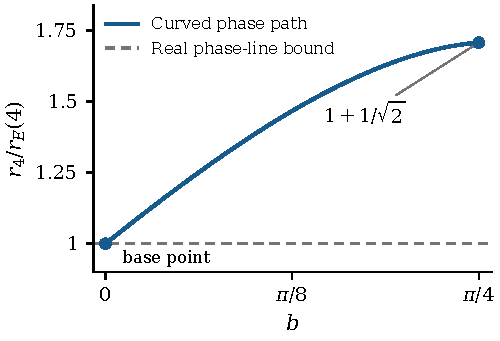
\includegraphics[width=\columnwidth]{figures/fig3_curved.pdf}
  \caption{Enhancement at $n=4$ along the explicit curved phase path.
  The solid curve is $r_4/r_E(4)=\cos[b+\delta(b)]-\sin\delta(b)$, evaluated from the closed-form root on $0\leq b\leq\pi/4$.
  It increases from $1$ to $1+1/\sqrt2$.
  The dashed level is the radius bound for all real phase lines through the specified base point. Plotting code was prepared with OpenAI Codex (GPT-6) assistance and checked against the stated formulas.}
  \label{fig:curved}
\end{figure}


The threshold $n=5$ has a geometric explanation within the fixed
phase representation.  At $n=3$ the specified measurement is locally
isolated.  At $n=4$ the regularity equations admit deformations, but
every admissible phase line fails to increase the radius.  A curved path
through the same point does increase it.

\begin{proposition}[Local rigidity at $n=3$]
\label{low:rigidity}
In the fixed Pauli-orbit representation, the specified EJM at $n=3$ is
isolated in a neighborhood of its phase vector, after removing the overall
phase.
\end{proposition}
Indeed, the seven independent phases give eight differences between signed
local components.  Seven of their derivatives have determinant
$1/4096$ at the specified point.  The inverse function theorem therefore
isolates the zero of these seven equations.  Since every signed component
equals $1/4$ at that point, the squared regularity conditions are equivalent
to signed equality in a neighborhood.  The exact Jacobian in
Appendix~\ref{low:app-rigidity} turns the numerical rank reported in
Ref.~\cite{PauwelsGisin2026} into an analytic local statement.

For $n=4$, write an arbitrary phase line as
\begin{equation}
 M_d(t)=C_4\operatorname{diag}
 \bigl(i^{f_0(z)}e^{itd_z}\bigr)H^{\otimes4},\qquad d_0=0.
 \label{low:line}
\end{equation}
The normalization $d_0=0$ removes only a common phase; the remaining
15 entries of $d$ are arbitrary real numbers.

Figure~\ref{fig:curved} compares the phase-line bound with the curved
enhancement described below.
\begin{theorem}[Phase lines and a curved enhancement at $n=4$]
\label{low:theorem}
Every line~\eqref{low:line} that remains a common-radius regular
tetrahedral measurement in a neighborhood of $t=0$ has
\begin{equation}
 r_d(t)=r_E(4)|\cos(\omega t)|\le r_E(4)
 \label{low:line-bound}
\end{equation}
for some real $\omega$.  Nevertheless, there is an explicit curved phase
path through the same measurement for which
\begin{equation}
 r_4\bigl([0,\pi/4]\bigr)
 =\left[r_E(4),\left(1+\frac1{\sqrt2}\right)r_E(4)\right],
 \label{low:curve-range}
\end{equation}
and the radius is strictly increasing along the path.
\end{theorem}

The obstruction to straight paths is stronger than the Boolean bound.
The full linearized constraint kernel is four dimensional; second-order
conditions eliminate one direction except for a single candidate ratio,
and a nonzero third-order term eliminates that candidate.  The remaining
directions form two planes, each giving only the cosine law
\eqref{low:line-bound}.  Their explicit classification is given in
Appendix~\ref{low:app-lines}.

To construct a path that can leave these planes, allow two independent
real parameters $b,\delta$ and set $\theta_z=bu_z+\delta v_z$, using the
two fixed integer masks $u,v$ in Eq.~\eqref{low:masks}.
For these phases, the signed physical Pauli components of the seed take
only two values: ten components equal $T/8$, whereas the components of
$X_1$ and $-Y_4$ equal $H/8$, where
\begin{align}
 T&=\cos(b+\delta)-\sin\delta,\nonumber\\
 H&=\cos b+2\sin\delta\cos b+4\sin b\cos b.
 \label{low:two-components}
\end{align}
These identities hold before a path is selected.  The signed regularity
condition is therefore $H=T$, a quadratic equation in $\tan(\delta/2)$.

The root branch through $(b,\delta)=(0,0)$ has the following closed
expression.  For $0\le b\le\pi/4$, define
\begin{align}
 A(b)&=\cos b(1+2\sin b),\nonumber\\
 B(b)&=2\cos b+\sin b+1,\qquad
 C(b)=2\sin b\cos b,\nonumber\\
 \delta(b)&=-2\arctan\frac{2C(b)}
 {B(b)+\sqrt{B(b)^2-4A(b)C(b)}}.
 \label{low:delta}
\end{align}
With this choice, the phase path and measurement are
\begin{equation}
 \begin{aligned}
 \theta_z(b)&=bu_z+\delta(b)v_z,\\
 M_4(b)&=C_4\operatorname{diag}
 \bigl(i^{f_0(z)}e^{i\theta_z(b)}\bigr)H^{\otimes4}.
 \end{aligned}
 \label{low:curve}
\end{equation}
Thus all signed components coincide on the entire explicit path.
Unitarity and the Pauli-orbit relation then give the complete measurement
and its fixed local tetrahedra.  Its common radius is
\begin{equation}
 r_4(b)=r_E(4)\bigl[\cos\bigl(b+\delta(b)\bigr)-\sin\delta(b)\bigr].
 \label{low:curve-radius}
\end{equation}
The radicand and denominator in Eq.~\eqref{low:delta} are strictly
positive on the closed interval $0\le b\le\pi/4$.
Appendix~\ref{low:app-curve} proves that the branch is well defined and
that its radius is strictly increasing throughout this interval.
Both angles vanish at $b=0$, so the original measurement is recovered
column by column.  At the other endpoint $\delta(\pi/4)=-\pi/4$, giving
the upper endpoint in Eq.~\eqref{low:curve-range}.
The curved path leaves the two planes of admissible line directions and
has $r'_4(0)=\sqrt3/6>0$.

The larger value $3r_E(4)$ already occurs at a different measurement at $n=4$ in Ref.~\cite{PauwelsGisin2026}.  The purpose of
Eq.~\eqref{low:curve} is to increase the radius through the specified
$f_0$ measurement and explain the required curvature.  The parameter
segment of that earlier family contains no measurement equivalent to
this specified point under local unitaries, qubit permutations, and
outcome relabeling.  Appendix~\ref{low:app-invariant} gives a short
certificate using the one-qubit spectrum and the sum of the three
$2|2$ purities.  Whether a larger regular-tetrahedral solution manifold
connects the two families remains open.

\section{Discussion}
\label{discussion:section}

The phase framework separates two tasks: a diagonal unitary supplies a complete orthogonal measurement, while the interference terms determine its local geometry. A fixed four-feature Boolean kernel makes these local terms coincide for every $n\ge5$, producing a continuous radius interval from $0$ to $2r_E(n)$. The classification of radius laws for Boolean phase lines shows that this endpoint is optimal within the full two-valued-generator model. For even $n\ge8$, cancellation of the mixed background terms places the known cosine family and the enhanced family in one genuinely two-dimensional measurement family. The results at $n=3$ and $n=4$ explain the lower-dimensional boundary of this picture: exact local rigidity at the specified point at $n=3$, and a distinction between straight and curved phase deformations at $n=4$. Throughout these constructions, the actual single-qubit reduced states provide the link between the algebraic phase conditions, fixed tetrahedral directions, and continuously variable single-qubit-versus-rest entanglement.

Two questions remain close to these results. At $n=4$, the specified straight segment of the larger-radius family in Ref.~\cite{PauwelsGisin2026} contains no measurement equivalent to our reference EJM under local unitaries and relabelings. Whether the curved branch constructed here connects to that family elsewhere in the regular tetrahedral phase space is unresolved. At $n=6$, the four-color model has only the two crossing branches near the reference point. A finer phase partition may allow a two-parameter family containing both branches; resolving this requires controlling additional mixed terms beyond those present in the model studied here.

\section{Conclusions}
\label{conclusions:section}

We have constructed a continuous family of elegant joint measurements for every integer $n\ge5$, with fixed local tetrahedral directions and common radius covering $[0,2r_E(n)]$ through the specified reference measurement. The upper endpoint is attained and optimal among all admissible phase lines with two-valued real generators in the fixed phase representation. A single four-feature mechanism thus gives continuous control of local polarization while preserving global orthogonality. The embedding of the enhanced and known cosine families for even $n\ge8$, together with the curved enhancement at $n=4$, further shows how compatible phase directions and the shape of the phase path determine the available deformations.

\begin{acknowledgments}
[To be added.]
\end{acknowledgments}

\section*{Data availability}
The analytic information supporting the conclusions is included in this article and its appendixes. The accompanying draft package contains the Lean sources, exact verification scripts, and figure-generation code.

\appendix
\section{Local formulas and the all-\texorpdfstring{$n$}{n} reduction}
\label{core:appendix}

\subsection{Gate pullbacks and the physical point correction}
\label{core:pullbacks}

Let $\mathbf e_j$ denote a binary unit vector and $T_j=\mathbf e_j\oplus\cdots\oplus\mathbf e_n$. Direct conjugation through the CNOT chain gives
\begin{align}
 S^\dagger X_1S&=X_1,\nonumber\\
 S^\dagger X_jS&=X_{j-1}X_j\quad(j>1),\nonumber\\
 S^\dagger Z_jS&=Z_jZ_{j+1}\cdots Z_n.
 \label{core:cnot-pullbacks}
\end{align}
Conjugating by the final-qubit Hadamard and using $Y=iXZ$ gives Table~\ref{core:pullback-table}. In $R=i^kX^aZ^b$, the $Z$ factors act first. For example, $Y_n$ pulls back to $-iX_{n-1}X_nZ_n$; the signed observable $-Y_n$ therefore has $\Gamma=-i$, as do the other class-I rows. Every row has $a\ne0$ and $h\ne0$.

\begin{table*}[t]
\caption{Pullbacks $C_n^\dagger\widetilde P C_n=i^kX^aZ^b$, expressed by $a$, $h=a\oplus b$, and $\Gamma=i^{k-|a|}$. The table is valid for every $n\ge2$; internal rows are absent at $n=2$.}
\label{core:pullback-table}
\begin{ruledtabular}
\begin{tabular}{ccccc}
Class&Signed observable&$a$&$h$&$\Gamma$\\
I&$X_1$&$\mathbf e_1$&$\mathbf e_1$&$-i$\\
I&$Y_1$&$\mathbf e_1\oplus\mathbf e_n$&$T_2$&$-i$\\
I&$Z_j$, $1\le j\le n$&$\mathbf e_n$&$T_j$&$-i$\\
I&$X_n$&$\mathbf e_{n-1}$&$T_{n-1}$&$-i$\\
I&$-Y_n$&$\mathbf e_{n-1}\oplus\mathbf e_n$&$\mathbf e_{n-1}$&$-i$\\
II&$X_j$, $2\le j<n$&$\mathbf e_{j-1}\oplus\mathbf e_j$&$\mathbf e_{j-1}\oplus\mathbf e_j$&$-1$\\
II&$Y_j$, $2\le j<n$&$\mathbf e_{j-1}\oplus\mathbf e_j\oplus\mathbf e_n$&$\mathbf e_{j-1}\oplus T_{j+1}$&$-1$\\
\end{tabular}
\end{ruledtabular}
\end{table*}

For any real $\Theta$, direct summation yields
\begin{equation}
 B_R=2^{-n}\Gamma\sum_z(-1)^{h\cdot z}
 e^{i[\Theta(z)-\Theta(z\oplus a)]}.
 \label{core:background-sum}
\end{equation}
Indeed, $i^{|z|-|z\oplus a|}=i^{-|a|}(-1)^{a\cdot z}$. Also,
\begin{equation}
 \bra{\chi_\Theta}R\ket0
 =2^{-n/2}\Gamma e^{-i\Theta(a)},\qquad
 \bra0R\ket0=0.
\end{equation}
Expanding Eq.~\eqref{core:defect-state} therefore proves Eq.~\eqref{core:signal}, including its normalization and its background term.

For completeness, the reference-phase identity follows from
\begin{equation}
 \sum_{\ell=0}^{w}(-1)^\ell\binom w\ell=0\quad(w>0).
\end{equation}
Removing the $\ell=0,1$ terms gives $f_0=w-1$ for $w>0$. At $z=0$, the bracket in Eq.~\eqref{core:defect-state} has amplitude $2^{-n/2}i$; multiplication by $-i$ restores the reference amplitude $2^{-n/2}$. At every other input it has amplitude $2^{-n/2}i^{f_0(z)}e^{i\Theta(z)}$. This proves the decomposition at the level of the actual input amplitudes.

\subsection{Boolean backgrounds and character pairing}
\label{core:pairing}

Put $\xi_z=2^{-n/2}i^{|z|}$ and $\eta_z=(-1)^{q(z)}\xi_z$. Since $q$ is Boolean,
\begin{equation}
 \ket{\chi_{tq}}=e^{it/2}
 \left[\cos(t/2)\ket\xi-i\sin(t/2)\ket\eta\right].
\end{equation}
Equation~\eqref{core:background-sum} gives
\begin{align}
 \bra\xi R\ket\xi&=0,\nonumber\\
 \bra\xi R\ket\eta&=\Gamma W_q(h),\nonumber\\
 \bra\eta R\ket\eta&=\Gamma W_{D_aq}(h).
\end{align}
In class I, $D_aq$ is invariant under translation by $a$, whereas $h\cdot a=1$. Its Walsh coefficient vanishes by pairing. The remaining cross term is $-\sin t\,W_q(h)$. In class II, $\Gamma=-1$ is real, so the cross term vanishes and the diagonal term is $-\sin^2(t/2)W_{D_aq}(h)$. This proves Eq.~\eqref{core:boolean-background} without requiring the background to vanish.

More generally, let $L:\mathbb F_2^n\to\mathbb F_2^k$ have rank $k$. If $h\notin\operatorname{row}L=(\ker L)^\perp$, there is a $w\in\ker L$ with $h\cdot w=1$. Translation by $w$ changes the sign of $(-1)^{h\cdot z}$ and leaves every function of $Lz$ unchanged. If $h=L^TH$, instead,
\begin{equation}
 2^{-n}\sum_z(-1)^{h\cdot z}G(Lz)
 =2^{-k}\sum_v(-1)^{H\cdot v}G(v),
 \label{core:compression}
\end{equation}
because every fiber has $2^{n-k}$ elements. This elementary pairing is the only general linear-encoding fact needed here.

\subsection{Exhaustive character classification for every \texorpdfstring{$n\ge5$}{n >= 5}}
\label{core:alln-classification}

For the four-feature map in Eq.~\eqref{core:features}, a physical character $h$ lies in its row space exactly when
\begin{equation}
 \begin{gathered}
 h\text{ is constant on }E_n\text{ and on }O_n,\\
 h_1=h_{n-1}\oplus h_n.
 \end{gathered}
 \label{core:row-test}
\end{equation}
Its four-bit representative is
\[
 H=(h_{n-1},h_E,h_O,h_n).
\]
The first condition tests the two internal parity features; the second follows because the coefficient of $z_1$ is the sum of the coefficients of $x$ and $s$. Conversely these conditions reconstruct the character from the four features. Both internal blocks contain a coordinate, so this representation is unique.

Applying Eq.~\eqref{core:row-test} to Table~\ref{core:pullback-table} gives exactly Table~\ref{core:residual-table}. Here and below, a four-bit integer uses $(x,b,c,s)$ in that order.

\begin{table}[tbp]
\caption{All local terms that survive character pairing for the four-feature map. $A=\mathcal L_na$, $h=\mathcal L_n^TH$. All rows absent from this table cancel before any property of $F$ is used.}
\label{core:residual-table}
\begin{ruledtabular}
\begin{tabular}{cccc}
Observable&Dimension&Class&$(A,H)$\\
$Y_1$&$n\ge5$&I&$(8,15)$\\
$Z_2$&$n\ge5$&I&$(1,15)$\\
$Z_{n-1}$&$n\ge5$&I&$(1,9)$\\
$X_n$&$n\ge5$&I&$(8,9)$\\
$Z_3$&$n=5$&I&$(1,11)$\\
$X_3$&$n=5$&II&$(6,6)$\\
$Y_3$&$n=5,6$&II&$(7,13)$\\
$Y_4$&$n=6,7$&II&$(7,11)$\\
\end{tabular}
\end{ruledtabular}
\end{table}

The classification follows directly from the supports of the characters. For class I, $X_1,Z_1,Z_n,-Y_n$ fail the endpoint relation in Eq.~\eqref{core:row-test}. The four dimension-independent rows in Table~\ref{core:residual-table} satisfy it and select complete parity blocks. An internal suffix $T_j$, $3\le j\le n-2$, can select complete blocks only for $n=5,j=3$. For $n\ge6$, $j=3$ selects $4$ and omits $2$; for $j\ge4$, the selected internal coordinate $n-2$ has the same parity as an omitted first block coordinate $2$ or $3$.

For class-II $X_j$, the endpoint cases $j=2,n-1$ fail the endpoint relation. Otherwise its character selects two neighboring internal coordinates. Both parity blocks can be fully selected only when each has one member, which gives $n=5,j=3$. For class-II $Y_j$, the support is $\{j-1\}\cup\{j+1,\ldots,n\}$. Again $j=2,n-1$ fail the endpoint relation. At $j=3$, the odd block must consist only of $3$, giving $n=5,6$. At $j=4$, the even block can contain no $6$, giving $n=6,7$. For $j\ge5$, the selected coordinate $j-1$ and the omitted first coordinate of the same parity violate block constancy. This proves the table for unbounded $n$.

To evaluate the surviving terms, the coefficient of $x$ in $F$ is $1\oplus s\oplus c$. All three characters $9,11,15$ have $x$ coefficient one, so summing over $x$ leaves only $c=s$. On the slices $c=s=0$ and $c=s=1$, respectively,
\begin{equation}
 F=1\oplus x\oplus b,\qquad F=x\oplus b.
\end{equation}
Characters $9$ and $11$ omit $b$, so their sums cancel over $b$. Character $15$ contributes $x\oplus b\oplus c\oplus s=x\oplus b$ on these slices, leaving opposite constant signs. These are the first three identities in Eq.~\eqref{core:six-cancellations}. Expanding $F(v)\oplus F(v\oplus A)$ gives Eq.~\eqref{core:derivatives}, whose $x$ dependence proves the other three. Thus all backgrounds vanish for all real $t$.

It remains to check the flips even when their characters have canceled. From Table~\ref{core:pullback-table}, class-I flips map into $\{1,8,9\}$, while class-II flips map into $\{6,7,10,11,12,13\}$. Direct substitution in the two branches of Eq.~\eqref{core:kernel} gives
\begin{equation}
 \begin{aligned}
 F(A)&=0\quad(A\in\{1,8,9\}),\\
 F(A)&=1\quad(A\in\{6,7,10,11,12,13\}).
 \end{aligned}
 \label{core:flip-values}
\end{equation}
These sets include both parities of the final internal coordinate. They prove the cross-term identities used in Theorem~\ref{core:unified-theorem}.

\subsection{Complete measurement, reduced states, and multiplicity}
\label{core:full-measurement}

The circuit obeys
\begin{equation}
 \begin{aligned}
 C_n^\dagger(Z_hZ_{h+1})C_n&=Z_h\quad(h<n),\\
 C_n^\dagger X^{\otimes n}C_n&=Z_n.
 \end{aligned}
\end{equation}
Since $D$ is diagonal and $H^{\otimes n}\ket{k}=Z^k\ket{+}^{\otimes n}$, these identities prove Eq.~\eqref{core:orbit} with the original column ordering $k=(e_1,\ldots,e_{n-1},\sigma)$. No parameter-dependent relabeling or column phase is needed. At site $j$, Pauli conjugation by the orbit element multiplies the physical $X,Y,Z$ expectations by $(-1)^{\kappa_j},(-1)^{\kappa_j+\sigma},(-1)^\sigma$, respectively. With the seed's orientation $\epsilon_j$, this gives Eq.~\eqref{core:vertices}.

For the actual partial trace $\rho_j=\operatorname{Tr}_{\bar j}\ket\psi\!\bra\psi$, one has $\operatorname{Tr}(\rho_j\sigma_\alpha)=\langle\psi|\sigma_{j\alpha}|\psi\rangle$. Normalization and the three Pauli components determine a $2\times2$ Hermitian matrix uniquely, proving Eq.~\eqref{core:bloch-orbit}. Each vector in Eq.~\eqref{core:vertices} has norm one. Two distinct labels change exactly two coordinate signs, so their dot product is $-1/3$.

For fixed $j$, $\kappa_j=e_{j-1}\oplus e_j$ is a nonzero linear functional of $e$, including $j=1,n$. It is independent of the column bit $\sigma$. Consequently each pair $(\kappa_j,\sigma)$ has exactly $2^{n-2}$ preimages. At positive radius these are four distinct reduced states; at zero radius they all equal $I/2$. Finally, unitarity of $M[D]$ proves both orthonormality and $\sum_k\ket{\psi_k}\!\bra{\psi_k}=I$. This closes the link from the phase kernel to a complete projective measurement.




\section{Proof of the sharp bounds for Boolean phase lines}
\label{bound:appendix}

This appendix proves Theorem~\ref{bound:theorem}: tetrahedral regularity fixes the signed local components, coefficient comparison gives the four radius laws, and low-dimensional character identities determine which laws are possible.

\subsection{From tetrahedral regularity to equal signed components}
The local action of the Pauli orbit sends a seed Bloch vector $(x,y,z)$
to the four vectors
\begin{equation}
 (x,y,z),\quad(-x,-y,z),\quad(x,-y,-z),\quad(-x,y,-z).
 \label{bound:orbit-four}
\end{equation}
The label map is onto these four sign patterns.  The three distinct
off-diagonal inner products are
$-x^2-y^2+z^2$, $x^2-y^2-z^2$, and $-x^2+y^2-z^2$.
They are equal precisely when $x^2=y^2=z^2$.
A common radius at all sites then makes the squares of all $3n$
signed components equal.  At the specified base point each signed
component equals $c_n>0$.  By continuity their signs remain positive
on a sufficiently small interval, and the components themselves are
equal there.

For Boolean $d$, every term in a local expectation has a phase
$e^{it[d(z)-d(z')]}$ with $d(z)-d(z')\in\{0,\pm1\}$.
Thus any difference of two signed components is
$A+B\cos t+C\sin t$.  If this vanishes near zero, its value and its
first two derivatives at zero give $A=B=C=0$.
Equality therefore holds for all real $t$, including any zero-radius
points.  Conversely, equal signed components give the regular orbit
in Eq.~\eqref{bound:orbit-four}, with radius
$\sqrt3\,|m_d|$.  This proves the local-to-global step used in
Theorem~\ref{bound:theorem}.

\subsection{Background terms and coefficient comparison}
Write $N=2^n$, $c=2/N$, and $q=d+\delta_0$.
Then $q$ is Boolean with $q(0)=1$, and Eq.~\eqref{core:defect-state}
applies with $\Theta=tq$. Combining the local formula
\eqref{core:signal} with the Boolean backgrounds in
Eq.~\eqref{core:boolean-background} gives the components for
classes I and II of Table~\ref{core:pullback-table}:
\begin{equation}
 m_I(t)=\begin{cases}
 c\cos t-W_q(h)\sin t,&q(a)=1,\\
 c-[c+W_q(h)]\sin t,&q(a)=0,
 \end{cases}
 \label{bound:component-i}
\end{equation}
and
\begin{equation}
 \begin{split}
 m_{II}(t)={}&-\tfrac12W_{D_aq}(h)(1-\cos t)\\
 &+c\bigl\{[1-q(a)]\cos t+q(a)(1-\sin t)\bigr\}.
 \end{split}
 \label{bound:component-ii}
\end{equation}

For $n\ge3$, both classes occur.  The cosine coefficient in
Eq.~\eqref{bound:component-i} forces all class-I flip values to equal
some $s\in\{0,1\}$.  The sine coefficient in
Eq.~\eqref{bound:component-ii} forces all class-II flip values to
equal some $k\in\{0,1\}$.  Comparing the sine coefficients across
the classes gives $W_q(h)=c(s+k-1)$, while comparing the constants
gives $W_{D_aq}(h)=2c(s+k-1)$.  The cosine coefficients then also
agree.  Substitution proves both directions of
Eq.~\eqref{bound:conditions} and yields the four laws.
Their maximum absolute values prove the general upper bound.

\subsection{Analytic exclusions at \texorpdfstring{$n=2,3,4$}{n=2,3,4}}
Use binary integers with $z_1$ the most significant bit.
For $n\ge3$ and every class-I character, the Walsh condition is equivalently
\begin{equation}
 \sum_z q(z)(-1)^{h\cdot z}=1-s-k.
 \label{bound:linear-character}
\end{equation}
Indeed, $W_q(h)=-2N^{-1}\sum_zq(z)(-1)^{h\cdot z}$ for $h\ne0$.

For $n=2$, only class I occurs and its flip masks cover all three
nonzero strings.  Equality of the cosine coefficients forces
$q(z)=s$ for every $z\ne0$.  The choices $s=0$ and $s=1$
give $q=\delta_0$ and $q\equiv1$, respectively.
Their common components are $c$ and $c\cos t$, so neither exceeds
the base radius in absolute value.

For $n=3$, the class-I flip masks are $\{1,2,3,4,5\}$ and
the class-II flip masks are $\{6,7\}$.
Thus $q(0)=1$, the first set has value $s$, and the second set
has value $k$; there are no further unknowns.
For $h=1$, the left side of Eq.~\eqref{bound:linear-character}
is $1-s$, which gives $k=0$.
For $h=4$, it is $1+s-2k$, which gives $2s-k=0$.
Hence $s=k=0$ and $d=0$.

For $n=4$, the class-I flip masks are $\{1,2,3,8,9\}$ and
the class-II masks are $\{6,7,12,13\}$.  Put
\begin{equation}
 (A,B,C,D,E,F)=(q_4,q_5,q_{10},q_{11},q_{14},q_{15}),
 \label{bound:unknown-values}
\end{equation}
where $q_j=q(j)$.  The four class-I characters $h=1,3,7,15$
give, respectively,
\begin{equation}
 \begin{aligned}
 A-B+C-D+E-F+k&=0,\\
 A-B-C+D-E+F+k&=0,\\
 -A+B-C+D+E-F+k&=0,\\
 -A+B+C-D-E+F+k&=0.
 \end{aligned}
 \label{bound:four-boundary-equations}
\end{equation}
Adding these equations gives $4k=0$ and therefore $k=0$.
Equation~\eqref{bound:four-laws} now leaves only $m=c$ or
$m=c\cos t$.  This exclusion covers every Boolean function at $n=4$; no ansatz for its support was used.
It is sufficient for the radius bound, so a list of individual
admissible supports is unnecessary.

The low-dimensional upper bounds are attained at $t=0$.
For every $n\ge5$, the explicit unified generator satisfies the
admissibility conditions and gives $m(-\pi/2)=2c_n$.
These two observations complete the proof of
Eq.~\eqref{bound:sharp-max}, with a maximum rather than merely a
supremum.

\section{Mixed backgrounds and the exception at \texorpdfstring{$n=6$}{n=6}}
\label{embed:appendix}

\subsection{Reduction to six finite identities}

We prove the joint-background cancellation used in Theorem~\ref{embed:theorem}. In this appendix, write $\mathcal B_R=2^n B_R$ for the unnormalized background expectation, where $B_R$ is the normalized quantity in Eq.~\eqref{core:signal}. For a pulled-back signed Pauli $R=i^pX^aZ^b$, put $h=a\oplus b$ and $\Gamma=i^{p-|a|}$. Equation~\eqref{embed:seed} gives
\begin{equation}
 \mathcal B_R=\Gamma\sum_z(-1)^{h\cdot z}
 u^{q_A(z)-q_A(z\oplus a)}
 v^{q_B(z)-q_B(z\oplus a)}.
 \label{embed:background-sum}
\end{equation}
The sign follows from
$i^{|z|-|z\oplus a|}=i^{-|a|}(-1)^{a\cdot z}$.

For class I, $a$ contains no even internal position, so the exponent of $u$ vanishes. The remaining $q_B$ expectation is zero by the unified-family calculation. Every class-II flip contains exactly one position $e\in E$. The $u$ exponents $1$ and $-1$ occur precisely on $z|_E=0$ and $z|_E=e_e$, respectively. Write
\begin{equation}
 \mathcal B_R=\Gamma\left[uK_+(v)+K_0(v)+u^{-1}K_-(v)\right].
 \label{embed:sectors}
\end{equation}
For class II, $h\cdot a=0$. Translation by $a$ exchanges the two nonzero sectors without changing the character and reverses the $v$ exponent. Hence
$K_-(v)=K_+(v^{-1})$. At $u=1$, the single-$q_B$ result gives $K_++K_0+K_-=0$. It is therefore enough to prove $K_+=0$.

On the positive sector, $q_B$ depends only on
\begin{align}
 w&=(z_1,c,z_{n-1},z_n),\qquad c=\bigoplus_{j\in O}z_j,\notag\\
 O&=\{3,5,\ldots,n-3\}.
 \label{embed:four-sector-bits}
\end{align}
If $h$ takes both values zero and one on $O$, choose two such positions. Flipping both preserves $c$, $q_B(z)$, and $q_B(z\oplus a)$, but reverses $(-1)^{h\cdot z}$. The corresponding terms cancel.

The following classification covers all internal observables when $n\ge8$. For $X_j$, $h=e_{j-1}\oplus e_j$. Only $j=2,n-1$ select no odd internal position; every other $j$ selects exactly one of the at least two positions in $O$. For $Y_j$,
$h=e_{j-1}\oplus\bigoplus_{k=j+1}^n e_k$. At $j=2,4$, its restriction to $O$ is all ones. At even $j\ge6$, it contains $j-1$ but omits $3$. At odd $j\le n-5$, it is a nonempty proper suffix of $O$. At $j=n-3,n-1$, it is zero. Consequently, only
\begin{equation}
 X_2,\ X_{n-1},\ Y_2,\ Y_4,\ Y_{n-3},\ Y_{n-1}
 \label{embed:six-remaining}
\end{equation}
remain after character pairing.

Here is an explicit finite certificate for these six terms, using only the four-feature kernel $F$ of Eq.~\eqref{core:kernel}. For $w=(w_1,w_2,w_3,w_4)$ define
\begin{equation}
 T_\varepsilon(w)=F(w_1\oplus w_3,\varepsilon,w_2,w_1\oplus w_4),
 \qquad\varepsilon\in\{0,1\}.
 \label{embed:restricted-kernel}
\end{equation}
Let $A$ encode the flip induced by $a$ on $w$ and let $H$ encode the remaining character. Both are written as four-bit integers, with $w_1$ the most significant bit. Then
\begin{equation}
 K_+(v)=2^{|O|-1}\sum_{w\in\mathbb F_2^4}
 (-1)^{H\cdot w}v^{T_0(w)-T_1(w\oplus A)}.
 \label{embed:finite-sector-sum}
\end{equation}
For $k=-1,0,1$, let $N_k^\pm$ count the inputs with exponent $k$ and character sign $\pm1$. Substitution of the two branches of $F$ gives the following complete counts; each entry is $(N_k^+,N_k^-)$:
\begin{center}
\small\setlength{\tabcolsep}{4pt}
\begin{tabular}{c rr ccc}
\hline\hline
Observable & $A$ & $H$ & $k=-1$ & $k=0$ & $k=1$\\
\hline
$X_2$ & 8 & 8 & $(3,3)$ & $(4,4)$ & $(1,1)$\\
$X_{n-1}$ & 2 & 2 & $(2,2)$ & $(6,6)$ & $(0,0)$\\
$Y_2$ & 9 & 15 & $(2,2)$ & $(6,6)$ & $(0,0)$\\
$Y_4$ & 5 & 7 & $(2,2)$ & $(6,6)$ & $(0,0)$\\
$Y_{n-3}$ & 5 & 3 & $(2,2)$ & $(6,6)$ & $(0,0)$\\
$Y_{n-1}$ & 3 & 1 & $(3,3)$ & $(4,4)$ & $(1,1)$\\
\hline\hline
\end{tabular}
\end{center}
Thus every coefficient in Eq.~\eqref{embed:finite-sector-sum} vanishes. Equations~\eqref{embed:sectors} and \eqref{embed:defect} give the common signed component $2^{1-n}(\cos\alpha-\sin\beta)$ for all even $n\ge8$. Unitarity and the orbit transfer in Eq.~\eqref{core:bloch-orbit} then establish the full measurement statement.

\subsection{The direct superposition at \texorpdfstring{$n=6$}{n=6}}

For $n=6$, $O=\{3\}$. The two additional terms $X_3,X_4$ both have $(A,H)=(4,4)$ in Eq.~\eqref{embed:finite-sector-sum}. Their counts for $k=-1,0,1$ are $(4,2),(4,4),(0,2)$, giving
\begin{align}
 K_+(v)&=2v^{-1}-2v,\notag\\
 K_-(v)&=-K_+(v),\qquad K_0(v)=0.
 \label{embed:six-sectors}
\end{align}
Since $\Gamma=-1$, the unnormalized backgrounds are
\begin{equation}
 \mathcal B_{X_3}=\mathcal B_{X_4}
 =2(u-u^{-1})(v-v^{-1})=-8\sin\alpha\sin\beta.
 \label{embed:six-mixed}
\end{equation}
The other sixteen backgrounds vanish. All eighteen defect contributions still equal $2(\cos\alpha-\sin\beta)$, so equal signed components are equivalent to $\sin\alpha\sin\beta=0$ for all real parameters. In a neighborhood of the base point, these are exactly the two coordinate axes. Changing only the zero-string phase cannot remove their difference: $X_2$ and $X_3$ belong to the same class and have identical defect terms.

\subsection{Four colors with an independent zero-string phase}

For a stronger local statement, allow arbitrary phases on the four values of $(q_A,q_B)$. After removing a global phase, write
\begin{equation}
 \lambda_{00}=1,\quad\lambda_{10}=e^{i\alpha},\quad
 \lambda_{01}=e^{i\beta},\quad\lambda_{11}=e^{i\gamma}.
 \label{embed:colors}
\end{equation}
The seed is
\begin{equation}
 \frac{-i}{8}C_6\left[\sum_z i^{|z|}\lambda_{q_A(z),q_B(z)}\ket z
 +(e^{i\phi}-e^{i\gamma})\ket{0^6}\right].
 \label{embed:color-seed}
\end{equation}
The base point is $(\alpha,\beta,\gamma,\phi)=(0,0,0,\pi/2)$. The direct superposition has $\gamma=\alpha+\beta$ and $\phi=\pi/2$.

The defect contributions before the factor $2/64$ are
\begin{align}
 F_I&=\sin(\phi-\alpha)-\sin(\gamma-\alpha),\notag\\
 F_{II}&=\cos(\gamma-\beta)-\cos(\phi-\beta).
 \label{embed:color-defect}
\end{align}
The complete unnormalized backgrounds follow from the finite sum
\begin{equation}
 \mathcal B_R=\Gamma\sum_{z\in\mathbb F_2^6}(-1)^{h\cdot z}
 \lambda_{q_A(z),q_B(z)}
 \overline{\lambda_{q_A(z\oplus a),q_B(z\oplus a)}}.
 \label{embed:color-sum}
\end{equation}
With the pullbacks of Table~\ref{core:pullback-table} and the explicit Boolean functions above, the only nonzero expressions are
\begin{align}
 \mathcal B_{X_3}=\mathcal B_{X_4}
 &=4[-\cos\alpha+\cos\gamma\notag\\[-2pt]
 &\hspace{1.4em}-\cos(\alpha-\beta)+\cos(\beta-\gamma)],\notag\\
 \mathcal B_{Y_3}&=8[\cos\alpha-\cos(\beta-\gamma)],\notag\\
 \mathcal B_{Z_4}=\mathcal B_{Z_5}=\mathcal B_{X_6}
 &=-8[\sin\beta+\sin(\alpha-\gamma)].
 \label{embed:color-backgrounds}
\end{align}
The other twelve expressions vanish identically. Thus each actual signed expectation is $(\mathcal B_R+2F_I)/64$ or $(\mathcal B_R+2F_{II})/64$, according to its class.

In particular, $X_1$ and $X_2$ have zero background and belong to classes I and II, respectively. Equal signed components therefore require $F_I=F_{II}$ and force each expression in Eq.~\eqref{embed:color-backgrounds} to vanish. Conversely, these conditions are sufficient. The background equations reduce to
\begin{align}
 \sin\beta&=\sin(\gamma-\alpha),\notag\\
 \cos\alpha&=\cos(\gamma-\beta),\notag\\
 \cos\gamma&=\cos(\alpha-\beta).
 \label{embed:color-equations}
\end{align}
Near the origin, the last equation gives $\gamma=\alpha-\beta$ or $\gamma=\beta-\alpha$. In the first case, the first equation gives $\sin\beta=-\sin\beta$, hence $\beta=0$ and $\gamma=\alpha$. In the second case, it gives $2\cos(\beta-\alpha)\sin\alpha=0$, hence $\alpha=0$ and $\gamma=\beta$. Both branches satisfy the middle equation.

Finally, let $G=F_I-F_{II}$. At the base point, $\partial_\phi G=-1$, and $\phi=\pi/2$ solves $G=0$ along both branches. The implicit function theorem makes this solution unique nearby. The complete local solution set is therefore
\begin{equation}
 (\alpha,0,\alpha,\pi/2)\quad\text{or}\quad(0,\beta,\beta,\pi/2).
 \label{embed:color-crossing}
\end{equation}
All signed components are positive at the base point. In a sufficiently small neighborhood, the fixed-orbit tetrahedral conditions with a common radius are consequently equivalent to equal signed components, as in Appendix B. Equation~\eqref{embed:color-crossing} therefore classifies the local regular measurements in the stated color model and proves Proposition~\ref{embed:six-proposition}.

\section{Low-dimensional proofs}
\label{low:appendix}

This appendix supplies the rigidity and curved-path proofs for Sec.~\ref{low:section}, followed by the invariant that distinguishes the specified four-qubit reference measurement from the known larger-radius segment.

\subsection{An exact rigidity certificate at \texorpdfstring{$n=3$}{n=3}}
\label{low:app-rigidity}

Write $b_z=i^{f_0(z)}$ and let $\theta_0=0$.  For a signed physical
Pauli operator $\widetilde P$, define the fixed matrix coefficients
\begin{equation}
 K_P(z,w)=\overline{b_w}b_z
 \langle w|C_n^\dagger\widetilde P C_n|z\rangle.
 \label{low:finite-coeff}
\end{equation}
The seed component and all its derivatives follow from the finite identity
\begin{equation}
 2^n m_P(\theta)=\sum_{z,w}K_P(z,w)e^{i(\theta_z-\theta_w)}.
 \label{low:finite-sum}
\end{equation}
In particular,
\begin{equation}
 2^n\partial_lm_P(0)
 =i\sum_{z,w}K_P(z,w)
 (\mathbf1_{z=l}-\mathbf1_{w=l}).
 \label{low:jacobian-formula}
\end{equation}
These formulas use the original circuit and therefore keep its signs and
normalization explicit.

For $n=3$, let $\mathcal F$ contain the eight differences $m_P-m_{X_1}$,
in the order
\begin{equation*}
 P=Y_1,Z_1,X_2,Y_2,Z_2,X_3,-Y_3,Z_3.
\end{equation*}
The columns correspond to $\theta_1,\ldots,\theta_7$.
Equation~\eqref{low:jacobian-formula} gives
\begin{equation}
 4D\mathcal F(0)=
 \begin{pmatrix}
 -2&-2&0&1&1&0&2\\
 -1&-2&0&-1&2&2&0\\
 -1&-1&-1&0&1&0&1\\
 -1&-1&-1&0&1&1&0\\
 -1&-2&0&1&0&0&2\\
 -2&-1&0&1&0&0&2\\
 0&-2&-1&1&2&0&0\\
 -1&0&-2&1&0&2&0
 \end{pmatrix}.
 \label{low:jacobian-three}
\end{equation}
The determinant of the first seven rows of the displayed integer matrix is
$4$.  Hence the corresponding derivative determinant is
$4/4^7=1/4096$.  The inverse function theorem applies to these seven
real analytic component differences and implies that their common zero is
locally unique.  Every regular-tetrahedral measurement sufficiently near
the specified point satisfies these equations: all signed components are
positive there, so equality of their squares implies equality of the
components themselves.  This proves Proposition~\ref{low:rigidity} in
the full seven-dimensional phase space.

\subsection{All real phase lines at \texorpdfstring{$n=4$}{n=4}}
\label{low:app-lines}

Let $\mathcal F$ now contain the eleven differences from $X_1$, with the
remaining signed operators ordered as
\begin{equation*}
 Y_1,Z_1,X_2,Y_2,Z_2,X_3,Y_3,Z_3,X_4,-Y_4,Z_4.
\end{equation*}
For a line $\theta=td$, Eq.~\eqref{low:finite-sum} gives the exact
derivative rule
\begin{equation}
 16\frac{d^k}{dt^k}m_P(td)\bigg|_{t=0}
 =\sum_{z,w}K_P(z,w)\bigl[i(d_z-d_w)\bigr]^k.
 \label{low:line-derivative}
\end{equation}
The first-order equations have precisely the following four-parameter
solution, where $a,b_*,c,\kappa$ are arbitrary real numbers:
\begin{equation}
 \begin{aligned}
 d_0&=0,\qquad d_1=d_2=d_9=a,\\
 d_3=d_8&=a-c,\qquad d_{10}=b_*-c,\\
 d_4=d_5&=-a+b_*-c/2+\kappa,\\
 d_6=d_7=d_{12}=d_{13}&=c,\\
 d_{11}&=b_*,\qquad d_{14}=d_{15}=\kappa.
 \end{aligned}
 \label{low:kernel-four}
\end{equation}
For completeness, this is an exact linear-algebra reduction of
Eq.~\eqref{low:jacobian-formula}: all four displayed directions annihilate
$D\mathcal F(0)$, and the minor of $16D\mathcal F(0)$ with columns
$(1,2,3,4,5,6,7,8,10,12,14)$ has determinant $65536$.
Thus its rank is $11$ and the displayed kernel is exhaustive.

Put $G_P(t)=16[m_P(td)-m_{X_1}(td)]$.  The second-order conditions from
Eq.~\eqref{low:line-derivative} include
\begin{align}
 G''_{Y_1}(0)&=-2c(2a-c),\nonumber\\
 G''_{Y_2}(0)&=4c(a-2b_*+2c).
 \label{low:second-order}
\end{align}
If $c\ne0$, their vanishing requires $a=c/2$ and $b_*=5c/4$.
The next condition becomes
\begin{equation}
 G''_{X_2}(0)=-\frac{c(c+4\kappa)}2=0,
\end{equation}
so $\kappa=-c/4$.  But the same derivative rule then gives
\begin{equation}
 G'''_{Y_1}(0)=-\frac{39c^3}{8}\ne0.
 \label{low:third-order}
\end{equation}
Consequently $c=0$.  The remaining necessary second-order condition is
\begin{equation}
 G''_{X_2}(0)=-8(a-b_*)(a-b_*-\kappa)=0.
 \label{low:two-planes}
\end{equation}
Define the three subsets of the integer input labels
\begin{align}
 \mathcal A&=\{1,2,3,8,9,10,11\},\nonumber\\
 \mathcal B&=\{1,2,3,8,9,14,15\},\nonumber\\
 \mathcal C&=\{4,5,14,15\}.
 \label{low:line-supports}
\end{align}
The branch $b_*=a$ gives $d=a\mathbf1_{\mathcal A}
+\kappa\mathbf1_{\mathcal C}$, whereas the branch
$\kappa=a-b_*$ gives $d=b_*\mathbf1_{\mathcal A}
+(a-b_*)\mathbf1_{\mathcal B}$.  Substitution into the finite sum
\eqref{low:finite-sum} gives, for every signed local Pauli operator and
either branch,
\begin{equation}
 16m_P(td)=e^{iat}+e^{-iat}.
 \label{low:planes-sufficient}
\end{equation}
This checks sufficiency for all real parameters, rather than merely to
finite order.  Hence all allowable directions are exactly
\begin{equation}
 \operatorname{span}_{\mathbb R}
 \{\mathbf1_{\mathcal A},\mathbf1_{\mathcal C}\}
 \ \cup\ 
 \operatorname{span}_{\mathbb R}
 \{\mathbf1_{\mathcal A},\mathbf1_{\mathcal B}\}.
 \label{low:line-classification}
\end{equation}
Local regularity implies the signed equations used above by positivity at
the base point.  Their differences along any real direction are finite
exponential sums, so equality on an open interval extends to the whole
line.  Equations~\eqref{low:planes-sufficient} and
\eqref{low:line-classification} establish the first part of
Theorem~\ref{low:theorem} without a restriction on the number of values
taken by $d$.

\subsection{The curved branch and its full monotonic interval}
\label{low:app-curve}

Equation~\eqref{low:masks} specifies all phases in Eq.~\eqref{low:curve}.
Its entries are indexed by $z=0,\ldots,15$, with the most significant
bit first.  Inserting $\theta_z=bu_z+\delta v_z$ into
Eq.~\eqref{low:finite-sum} gives precisely the two expressions
in Eq.~\eqref{low:two-components}.  In particular, these identities
hold for independent real $b,\delta$, before any branch is selected.

\begin{equation}
 \begin{array}{c|rrrrrrrr}
 z&0&1&2&3&4&5&6&7\\
 u_z&0&1&1&1&2&2&0&0\\
 v_z&0&1&1&0&1&1&1&1\\[2pt]
 z&8&9&10&11&12&13&14&15\\
 u_z&1&1&0&0&0&0&1&1\\
 v_z&0&1&0&1&1&1&0&0
 \end{array}
 \label{low:masks}
\end{equation}

Set $q=-\delta$ and $z=\tan(q/2)$; the letter $z$ denotes a real
variable only in the following branch calculation.  The half-angle
identities give
\begin{equation}
 H-T=\frac{2(Az^2-Bz+C)}{1+z^2}.
 \label{low:quadratic-identity}
\end{equation}
We now verify the root in Eq.~\eqref{low:delta}, including its entire
domain.  Put $x=\tan(b/2)$ and $k=\sqrt2-1$.  Then
\begin{equation}
 Az^2-Bz+C=\frac{x+1}{(1+x^2)^2}F(x,z),
 \label{low:halfangle-polynomial}
\end{equation}
where
\begin{align}
 F(x,z)={}&-x^3z^2+x^3z-3x^2z^2-3x^2z-4x^2\nonumber\\
 &+3xz^2+xz+4x+z^2-3z.
 \label{low:polynomial}
\end{align}
On the square $0\le x,z\le k$, one has
\begin{equation}
 F_{xx}=6z[x(1-z)-(1+z)]-8<0.
\end{equation}
Using $k^2+2k-1=0$ and $4-12k<0$, it follows that
\begin{align}
 F_x(x,z)&\ge F_x(k,z)
 =4-8k+(4-12k)z\nonumber\\
 &\ge20k-8=20\sqrt2-28>0.
 \label{low:fx-positive}
\end{align}
The other derivative satisfies
\begin{align}
 F_z&=2z(1+3x-3x^2-x^3)+x^3-3x^2+x-3\nonumber\\
 &\le2k(1+3k)+k^3+k-3
 =5-4\sqrt2<0.
 \label{low:fz-negative}
\end{align}
The boundary values obey
\begin{align}
 F(x,x)&=-x(1+x^2)(x^2+2x-1)\ge0,\nonumber\\
 F(x,k)&\le F(k,k)=0.
 \label{low:boundary}
\end{align}
Thus each $x\in[0,k]$ has a unique root $z(x)\in[x,k]$;
$z(0)=0$, $z(k)=k$, and $x<z(x)<k$ in the interior.
At the root, $F_z<0$.  Since $A>0$, the corresponding quadratic has
positive discriminant and this is its smaller root.  Rationalizing that
root gives
\begin{equation}
 z(x)=\frac{2C}{B+\sqrt{B^2-4AC}},
 \label{low:root-identified}
\end{equation}
which is well defined also at $x=0$.  This proves the stated closed
formula rather than defining the path by an implicit existence argument.

Differentiating the now-identified simple root gives
$z'(x)=-F_x/F_z>0$.  Consequently $q'(b)>0$ and
$b\le q(b)\le\pi/4$.  With $T=\cos(b-q)+\sin q$,
\begin{equation}
 T'(b)=\sin(q-b)+q'(b)\,[\cos q-\sin(q-b)]>0.
 \label{low:monotone}
\end{equation}
The bracket is strictly positive: equality would require both
$q=\pi/4$ and $b=0$, inconsistent with the determined endpoint values.
The first term is nonnegative.  Finally,
$T(0)=1$ and $T(\pi/4)=1+1/\sqrt2$ prove the exact image
\eqref{low:curve-range}.  At the origin,
$z'(0)=4/3$, $q'(0)=4/3$, and $r'_4(0)=\sqrt3/6$.

Setting $n=4$ and $m=T/8$ in Eq.~\eqref{core:bloch-orbit} gives all
reduced states, with each fixed tetrahedral direction occurring four times.
The unitary factorization in Eq.~\eqref{low:curve} gives a complete
orthonormal measurement, and $b=0$ recovers the specified $D_{f_0}$.

\subsection{Non-equivalence of the reference measurement to the known \texorpdfstring{$n=4$}{n=4} segment}
\label{low:app-invariant}

We show that the specified reference measurement is not equivalent, under local unitaries, qubit permutations, or outcome relabeling, to any measurement on the $n=4$ segment in Appendix C of Ref.~\cite{PauwelsGisin2026}.
With $a\in[0,\pi/3]$, let $x=e^{ia}$ and write its input phases as
$i^{f_z}x^{k_z}$.  In order $z=0,\ldots,15$, the two fixed vectors are
\begin{align}
 f={}&(0,0,0,3,0,0,1,0,\nonumber\\
 &\hspace{12mm}0,0,0,2,0,1,3,3),\nonumber\\
 k={}&(0,1,-1,-1,0,1,0,0,\nonumber\\
 &\hspace{12mm}-1,2,0,1,3,3,1,0).
 \label{low:f159-data}
\end{align}
Here $a=\pi(1-\tau)/3$ in the parameterization of that reference.
The seed $C_4(i^{f_z}x^{k_z})_z/4$ has one-qubit eigenvalues
$(1\pm\sqrt3\,c(x))/2$, where
\begin{equation}
 c(x)=\frac{x^3+x^{-3}+2x+2x^{-1}}{16}
 =\frac{\cos3a+2\cos a}{8}.
 \label{low:f159-component}
\end{equation}
This is nonnegative on the stated segment, decreases from $3/8$ to
zero, and gives the already known endpoint $3r_E(4)$.

For a pure state at $n=4$ define
\begin{equation}
 S(\psi)=\operatorname{Tr}(\rho_{12}^{2})
 +\operatorname{Tr}(\rho_{13}^{2})
 +\operatorname{Tr}(\rho_{14}^{2}).
 \label{low:purity-invariant}
\end{equation}
The sum is invariant under local unitaries and qubit permutations:
complementary subsystems of a pure state have identical nonzero spectra,
so a permutation only permutes the three unordered $2|2$ terms.
Each column of a Pauli-orbit measurement shares these invariants with
its seed.  Outcome relabeling therefore cannot change the comparison.
At the specified $f_0$ point the three purities are
$(63,39,39)/128$, and hence $S_0=141/128$.

An equivalent measurement must have both the same one-qubit spectrum
and the same $S$.  On this segment these conditions require $c=1/8$
and $S=141/128$, respectively. Evaluating the reduced-state purities
from the amplitudes in Eq.~\eqref{low:f159-data} and clearing
denominators, with $x\ne0$, gives the necessary equations
$P(x)=Q(x)=0$, with
\begin{align}
 P(x)={}&x^6+2x^4-2x^3+2x^2+1,\nonumber\\
 Q(x)={}&6x^{16}-3x^{14}+74x^{12}+48x^{10}\nonumber\\
 &+134x^8+48x^6+74x^4-3x^2+6.
 \label{low:invariant-polynomials}
\end{align}
The Euclidean algorithm excludes a common root. Its first remainder is
\begin{equation}
 \begin{aligned}
 Q\bmod P={}&816x^5-2340x^4+2168x^3\\
 &-1240x^2+616x-596,
 \end{aligned}
\end{equation}
whose gcd with $P$ is $1$.  Thus the original parameter segment
contains no measurement equivalent to the specified $f_0$ measurement
under the allowed operations.






\bibliography{references}
\end{document}
